\providecommand{\main}{../../../..}
\documentclass[\main/dresen_thesis.tex]{subfiles}
\begin{document}
  \label{sec:looselyPackedNS:bilayerStacks:xrr}
  \begin{figure}[tb]
    \centering
    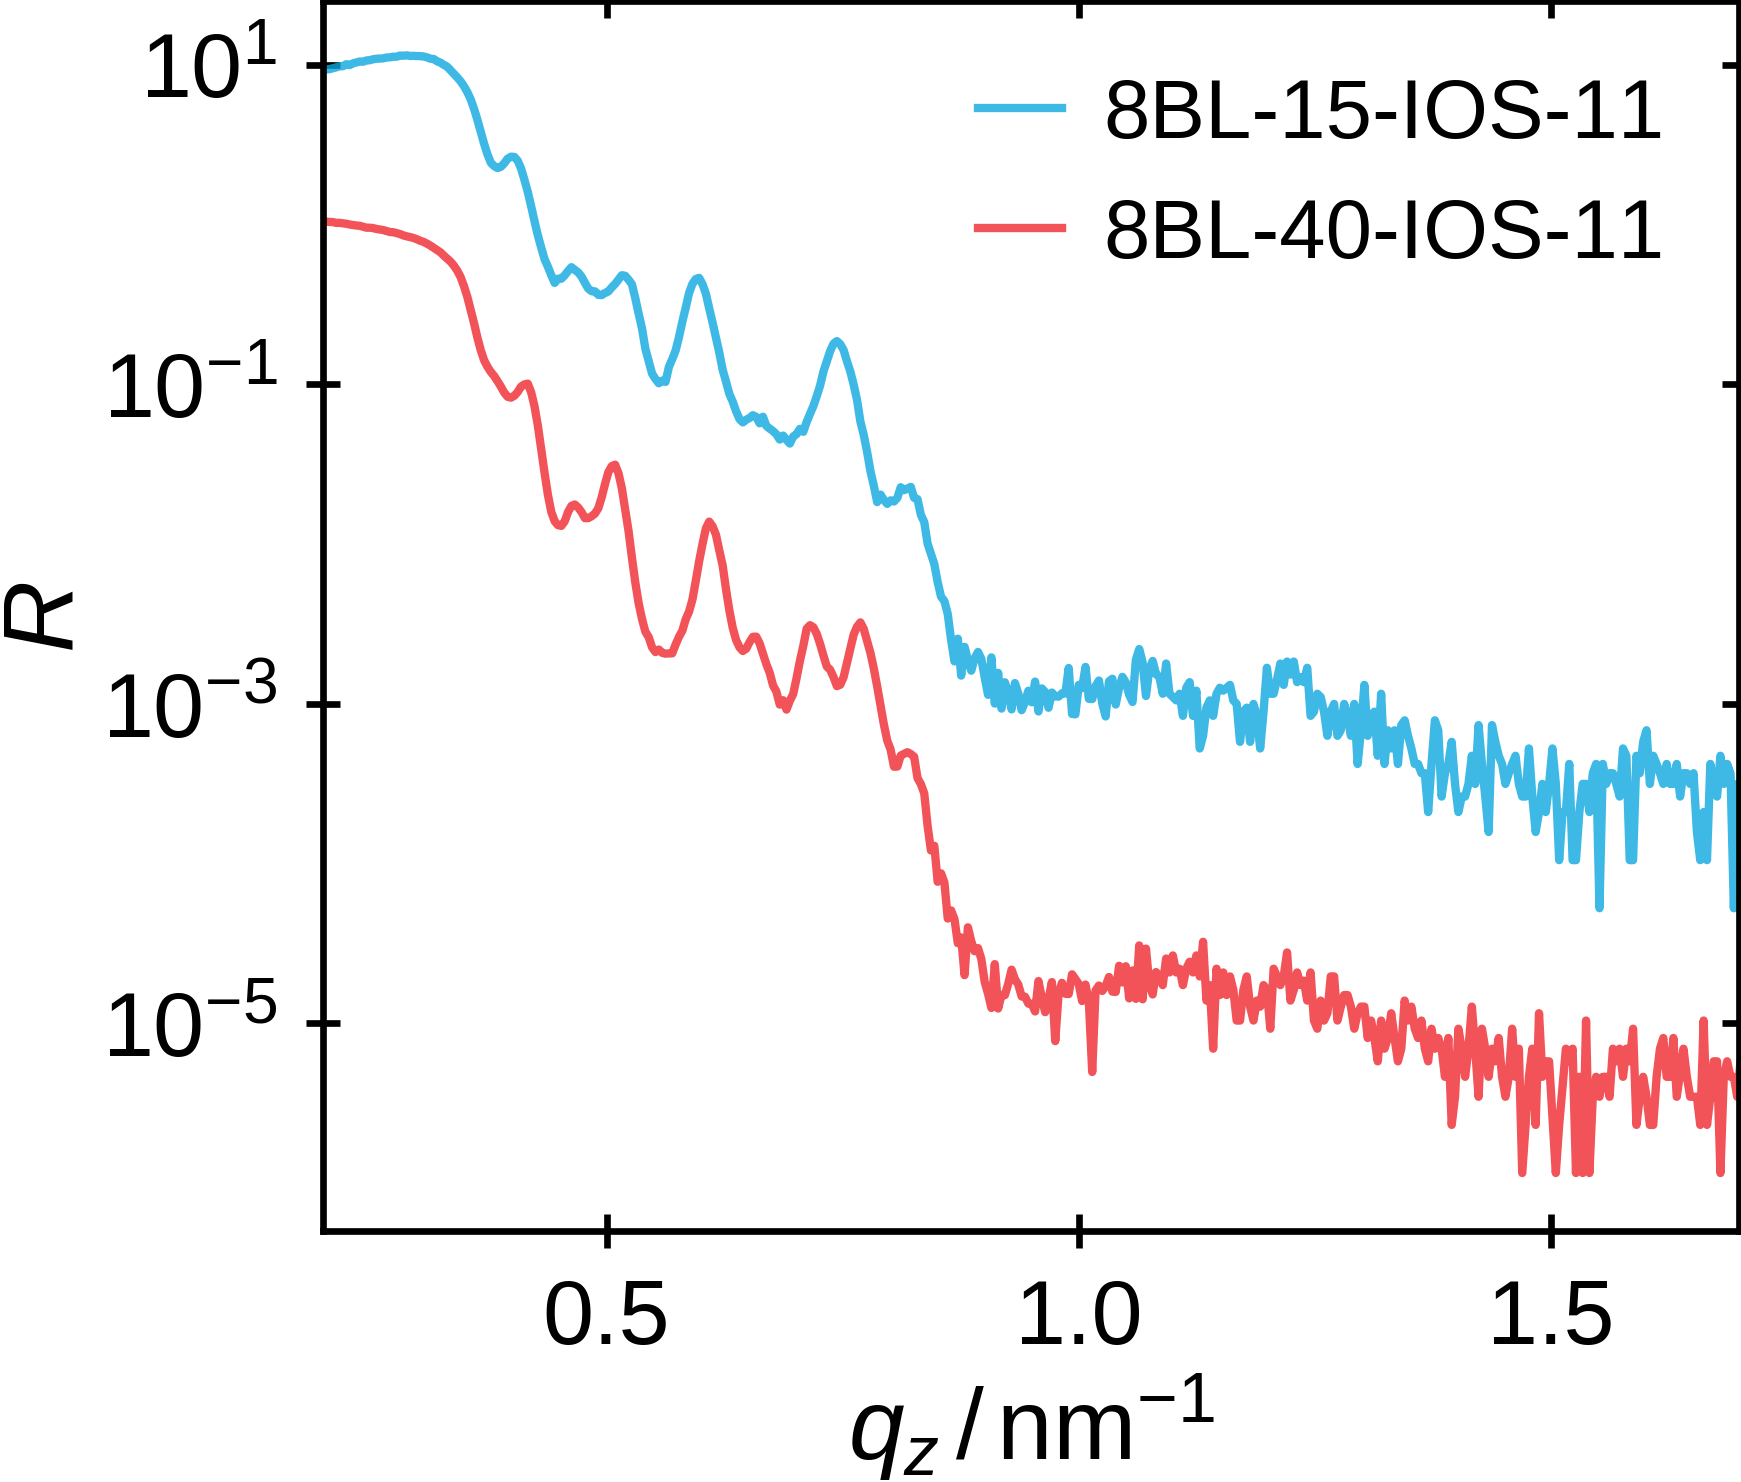
\includegraphics{looselyPackedNP_BilayersXRR_compareIOS11}
    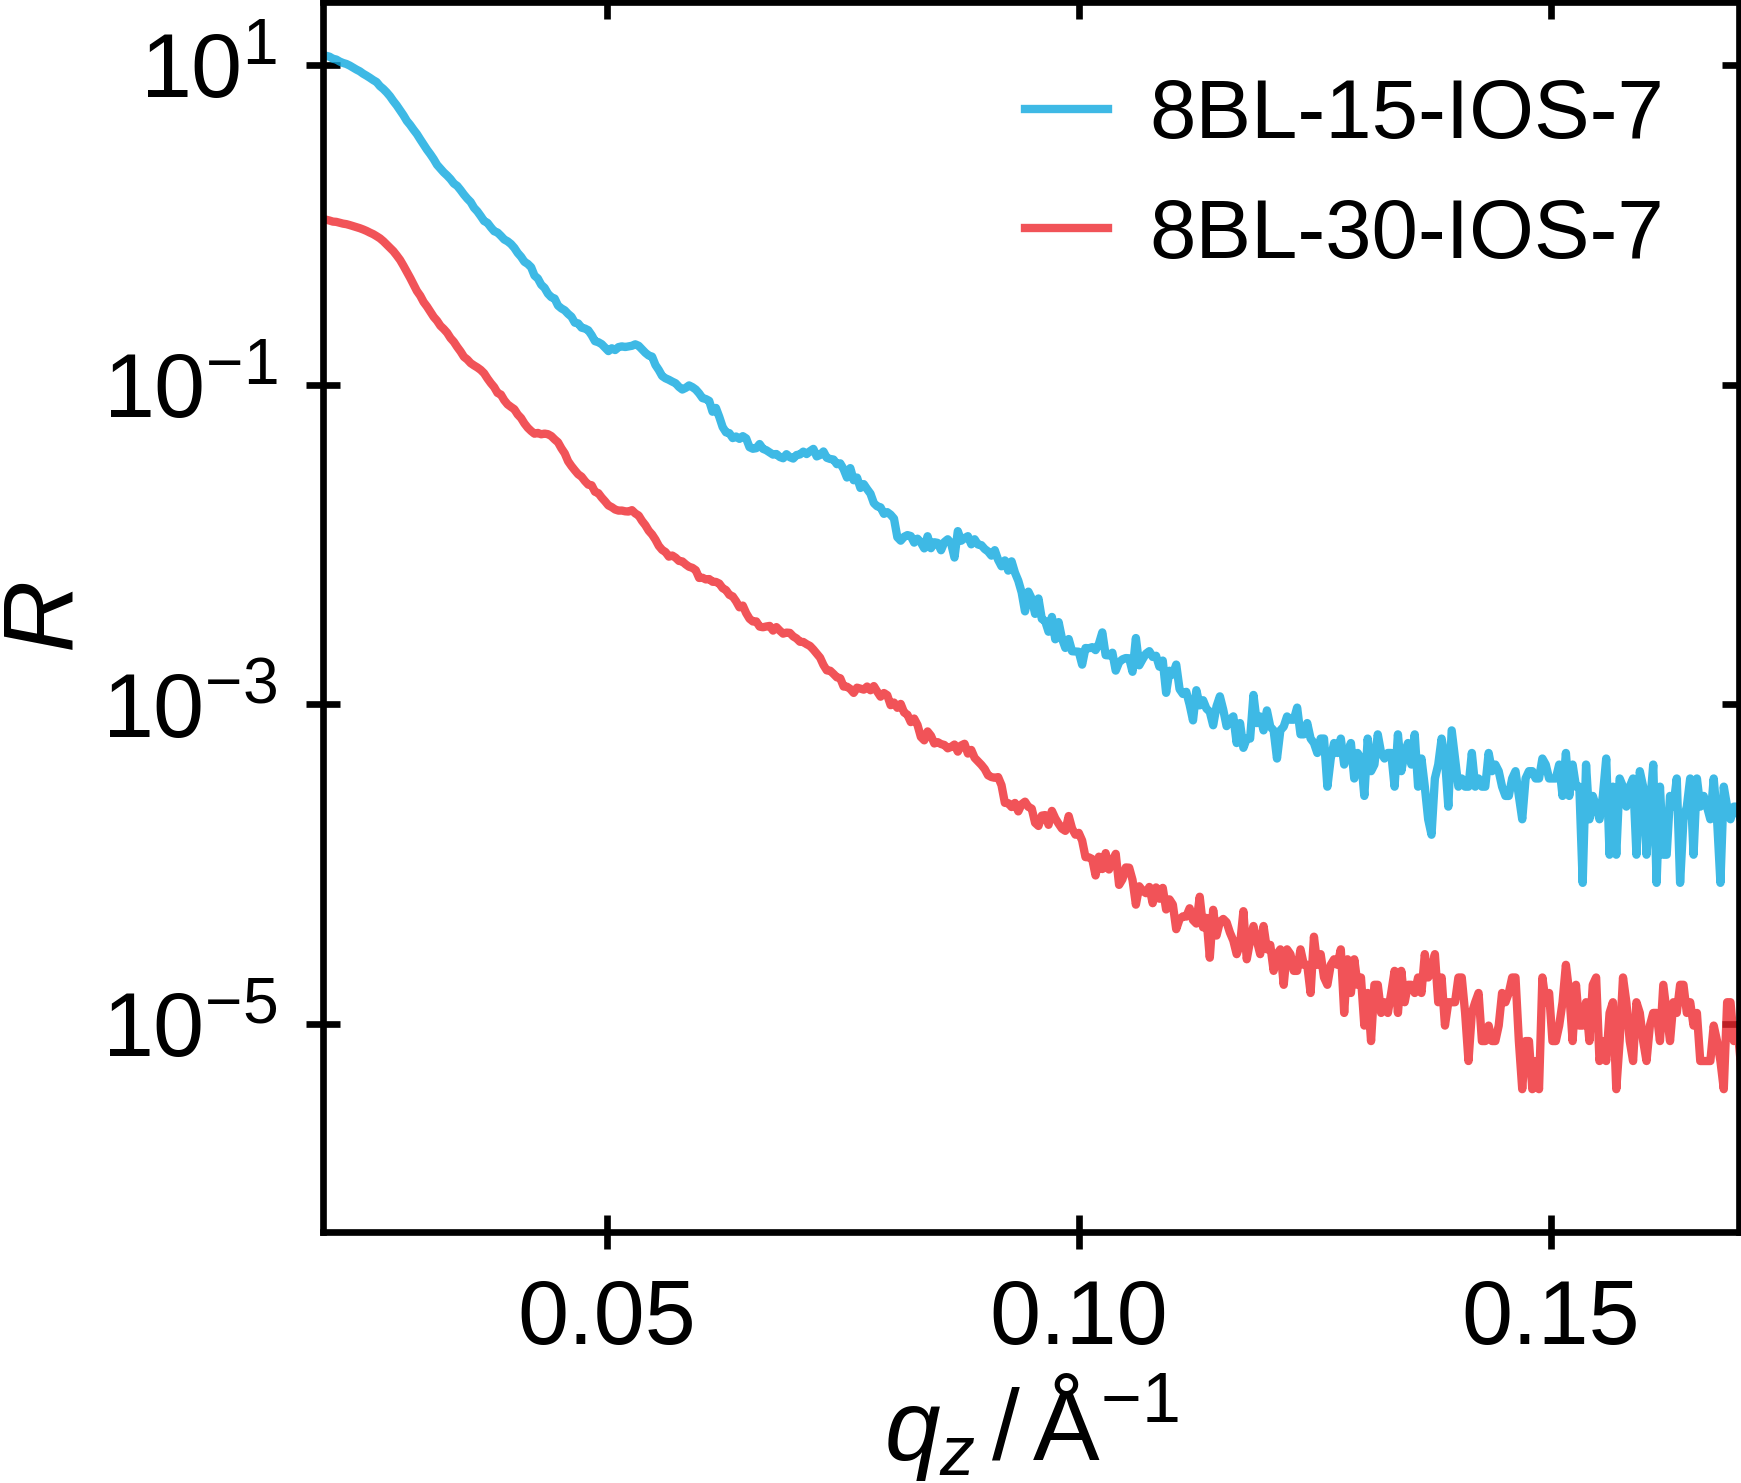
\includegraphics{looselyPackedNP_BilayersXRR_compareIOS7}
    \caption{\label{fig:looselyPackedNS:bilayerStacks:xrr}XRR data of the bilayer stacks 8BL-x-IOS-11 (left) and 8BL-x-IOS-7 (right) after footprint correction. The reflectivities of the varied PMMA thickness layers are shifted by a factor of ten for better visibility.}
  \end{figure}

  Using X-Ray reflectometry the layered structure of the bilayer stacks is probed on a macroscopic area of the sample, which enables to evaluate the sample quality on a quantitative level.
  In \reffig{fig:looselyPackedNS:bilayerStacks:xrr}, the reflectivity of the four bilayer stacks are shown.

  For the samples from IOS-7 in the right figure, no clear reflection peaks are observed for both bilayer stacks, but only weak oscillations are visible on the monotonously decreasing reflectivity in both cases.
  The samples 8BL-x-IOS-11 on the other hand, show well defined peaks in the reflectivity, which can be used to determine periodicity of the bilayer stack.


  \begin{figure}[tb]
    \centering
    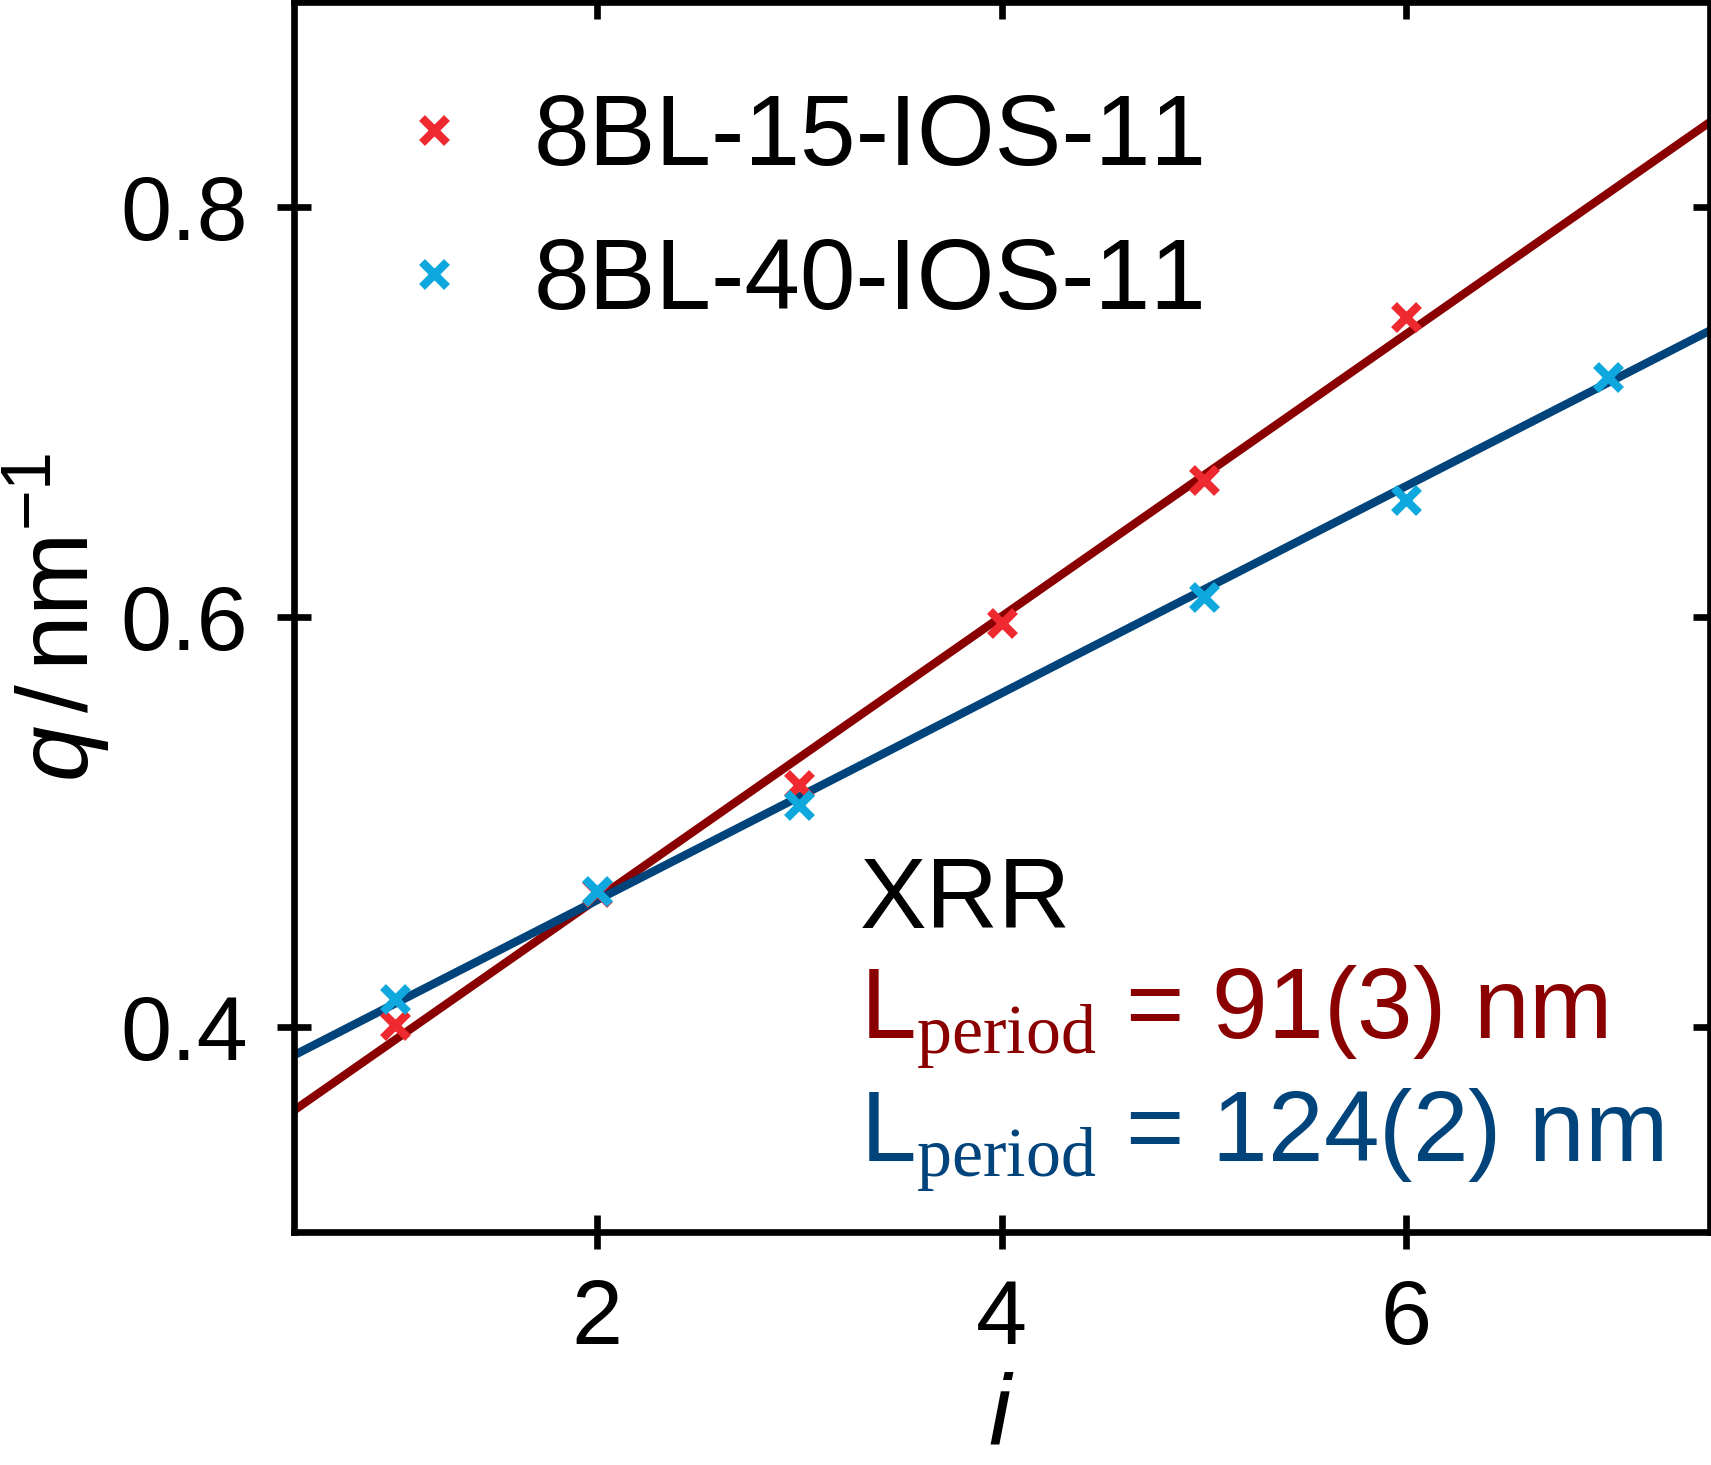
\includegraphics{looselyPackedNP_BilayersXRR_PeakPositions}
    \caption{\label{fig:looselyPackedNS:bilayerStacks:xrrPeaks}Peak positions of the 8BL-x-IOS-11 samples used to determine the length scale of the bilayer period.}
  \end{figure}

  In \reffig{fig:looselyPackedNS:bilayerStacks:xrrPeaks}, the maxima positions are plotted with respect to an incrementally increasing index and a linear fit through the points is shown from which the periodic length scales are determined.
  For 8BL-15-IOS-11 a greater slope is observed in comparison to 8BL-40-IOS-11, which correlates with the expected smaller PMMA thickness in this sample.
  The X-ray reflectivity reveals an average period of $91(3) \unit{nm}$ for 8BL-15-IOS-11 and $124(2) \unit{nm}$ for 8BL-40-IOS-11.
  In comparison to the result from SEM, where a periodic length of $63(5) \unit{nm}$ and $93(4) \unit{nm}$ is observed respectively, the XRR results show a larger average thickness for the bilayer stack both by $30 \unit{nm}$.

  \begin{figure}[tb]
    \centering
    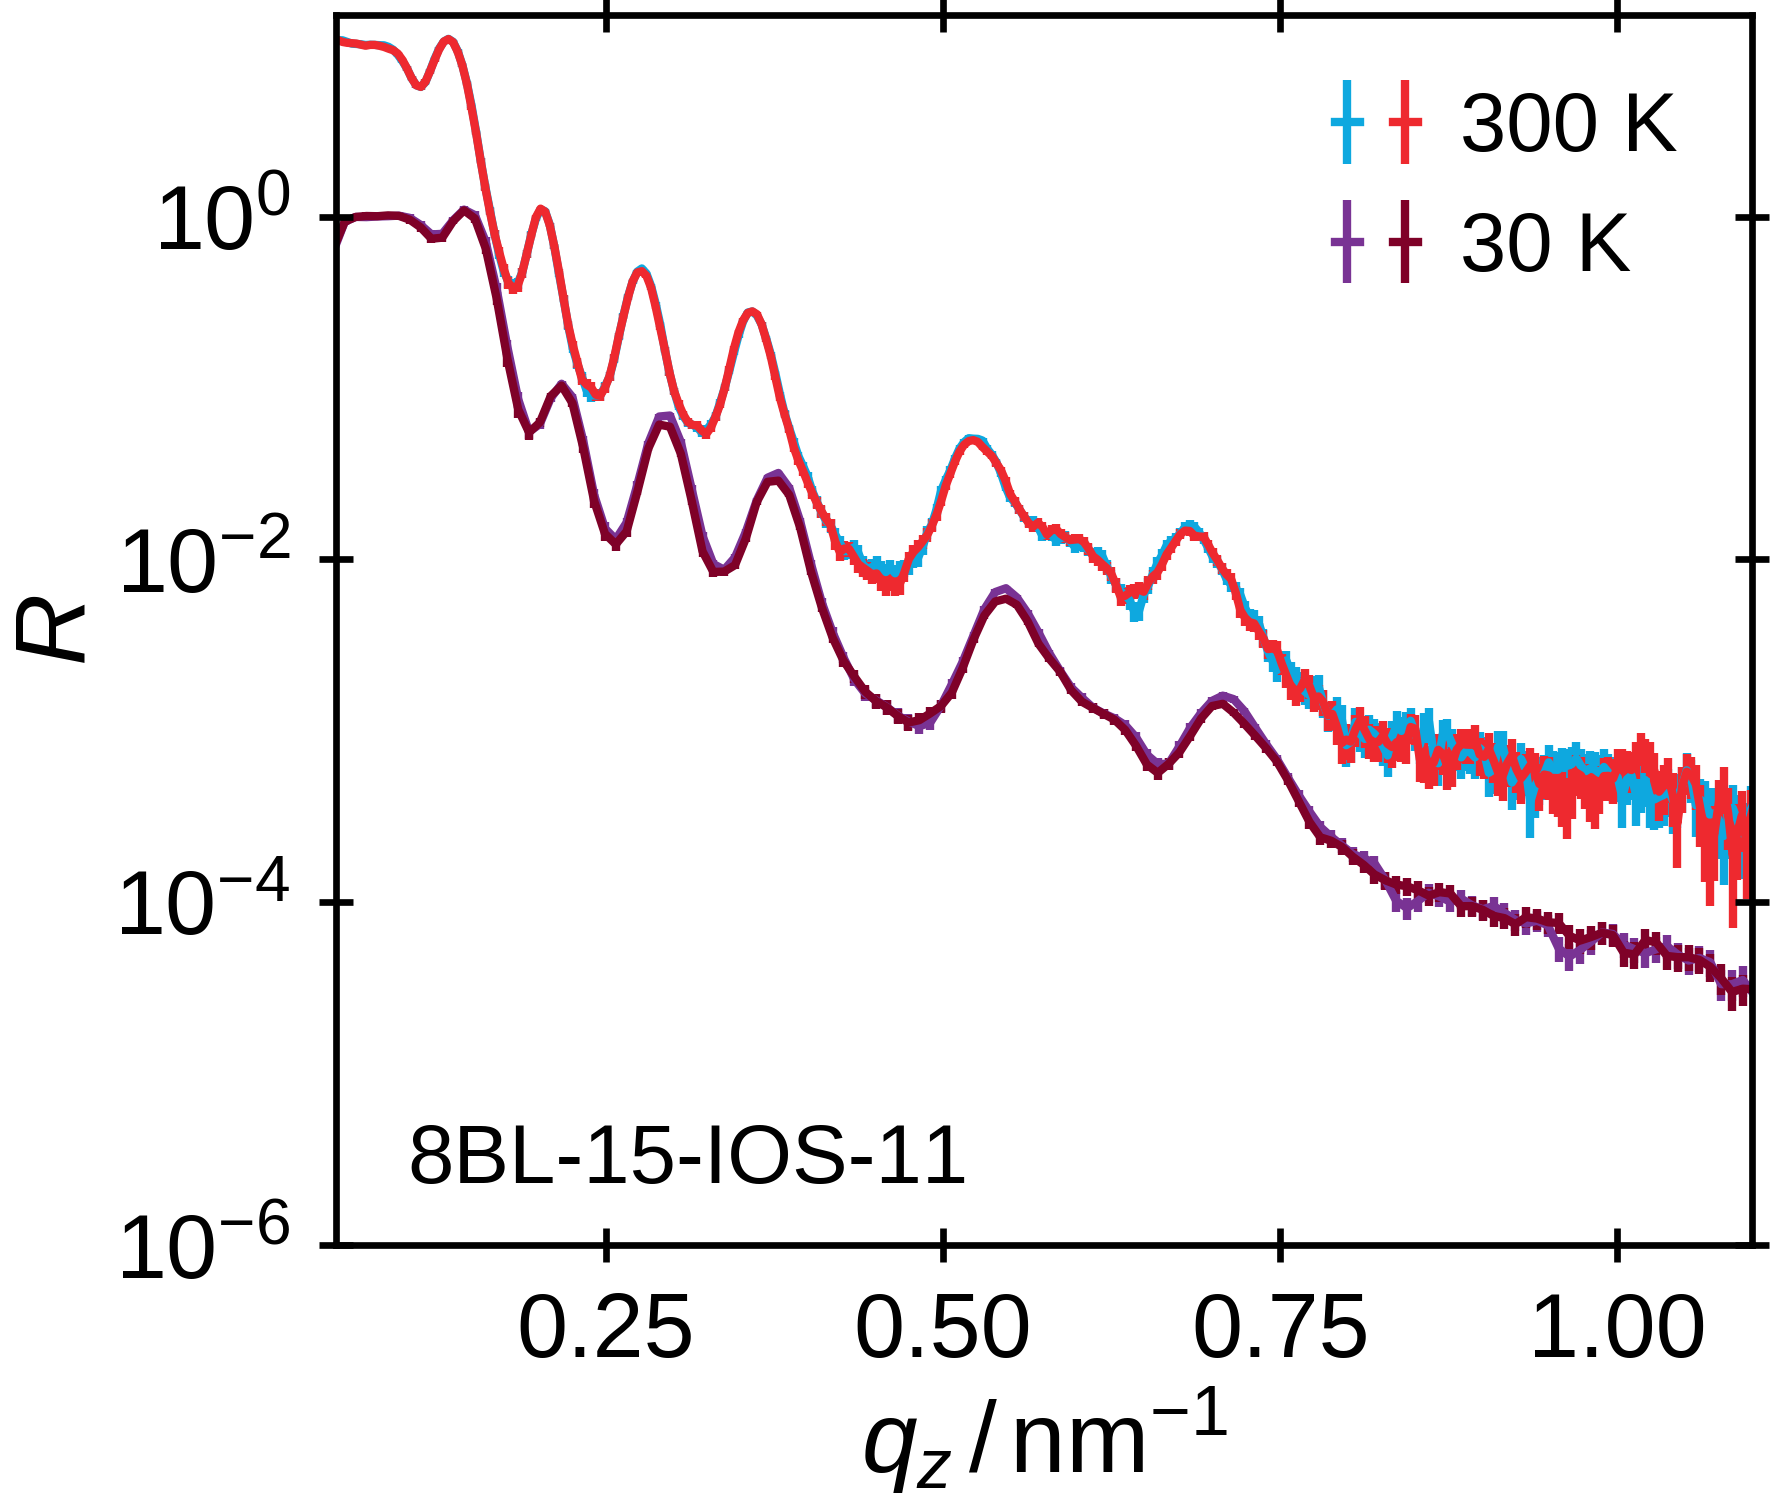
\includegraphics{looselyPackedNP_VerticalStructure_8BL-15-IOS-11_PNRCompare30K300K}
    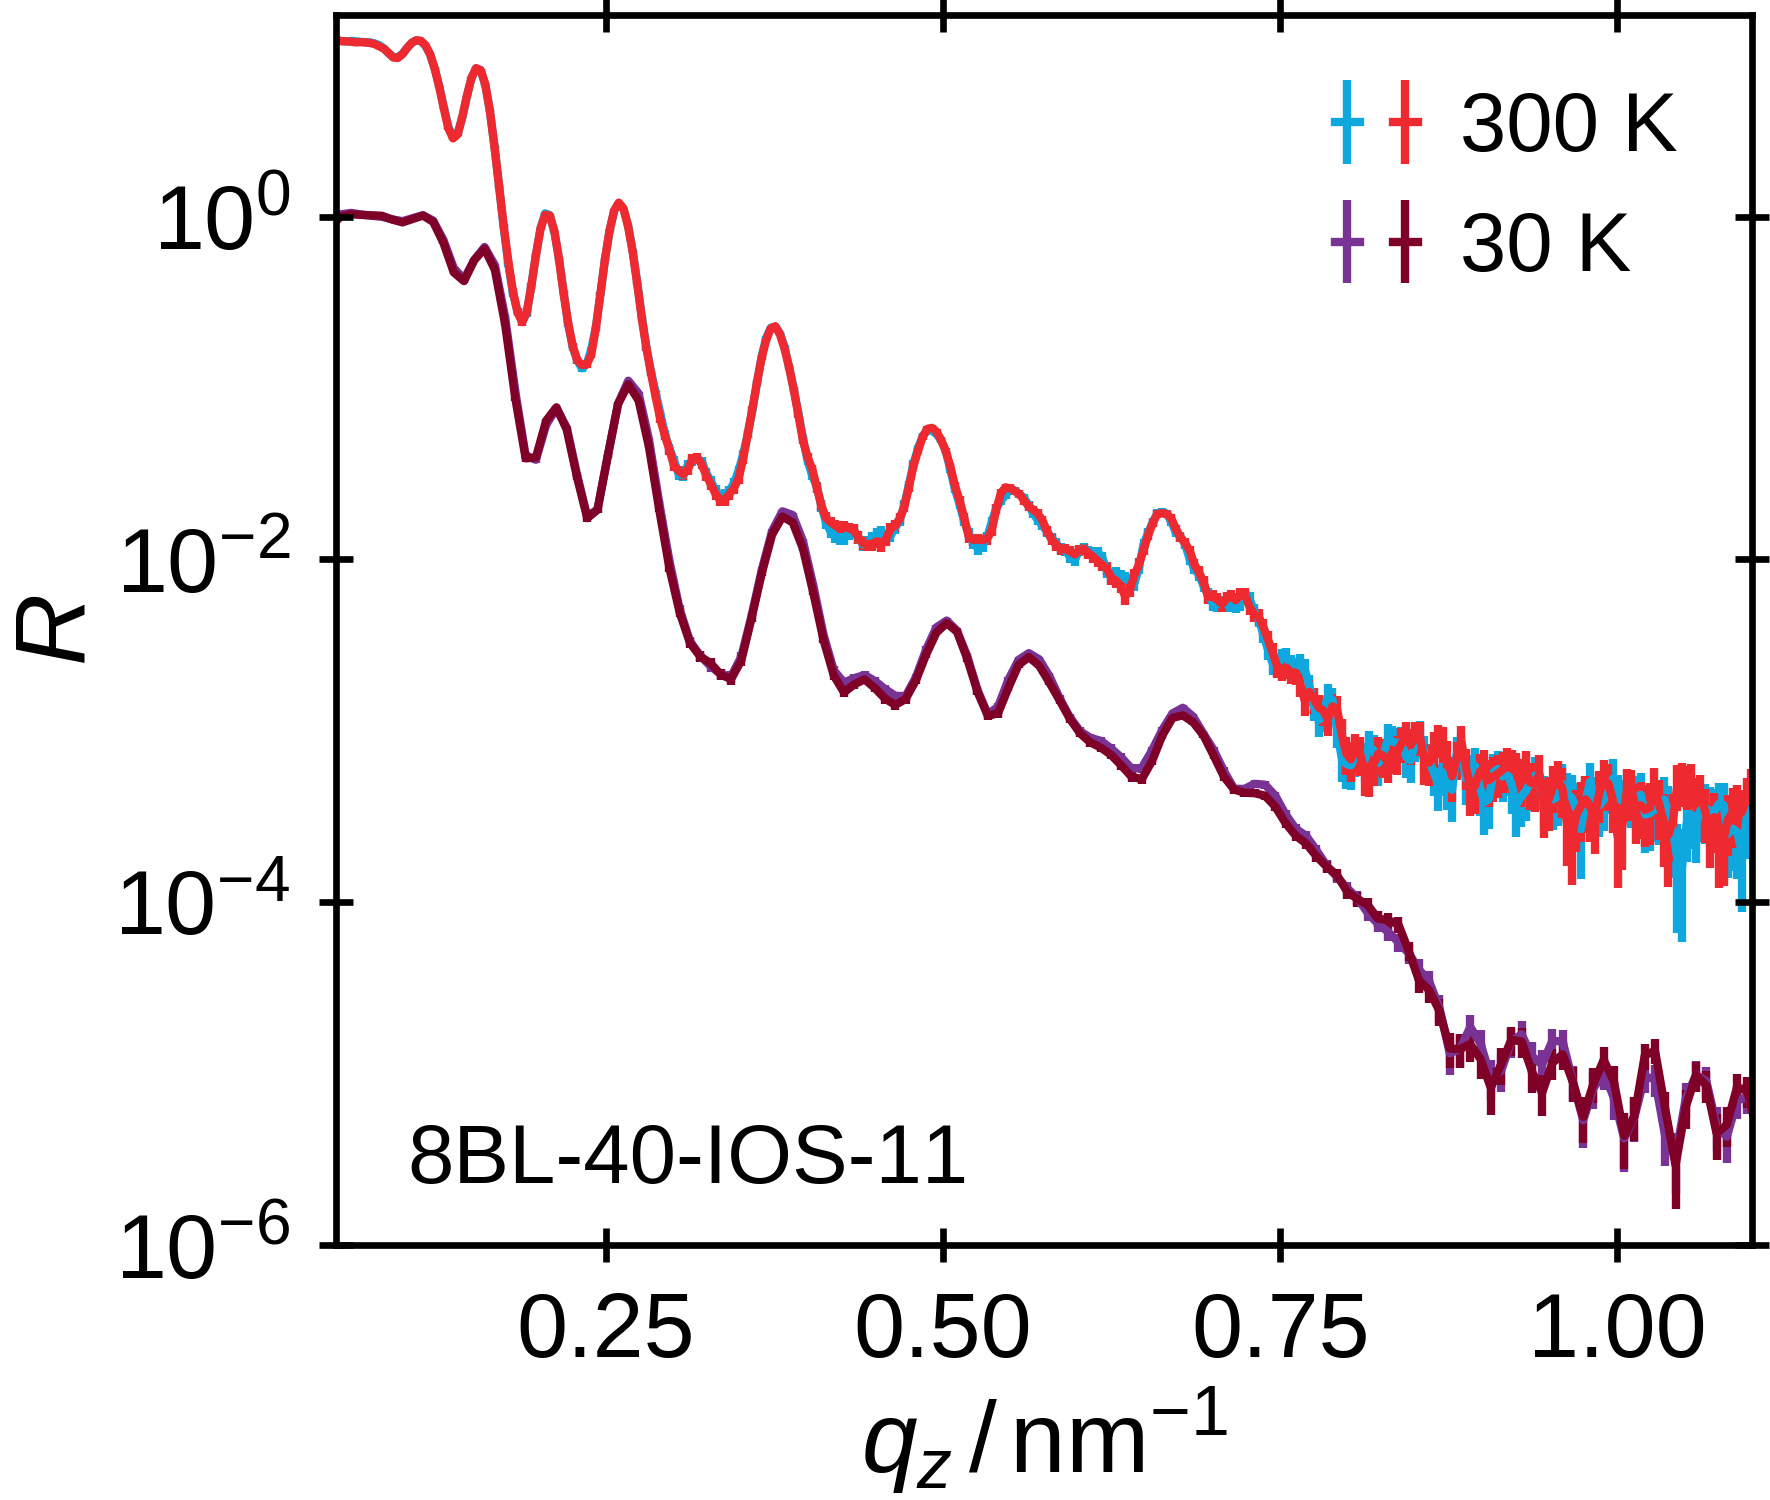
\includegraphics{looselyPackedNP_VerticalStructure_8BL-40-IOS-11_PNRCompare30K300K}
    \caption{\label{fig:looselyPackedNS:bilayerStacks:nr300K8BLIOS11}Neutron reflectivity data of the bilayer stacks 8BL-15-IOS-11 (left) and 8BL-40-IOS-11 (right) after footprint correction.}
  \end{figure}

  \begin{figure}[tb]
    \centering
    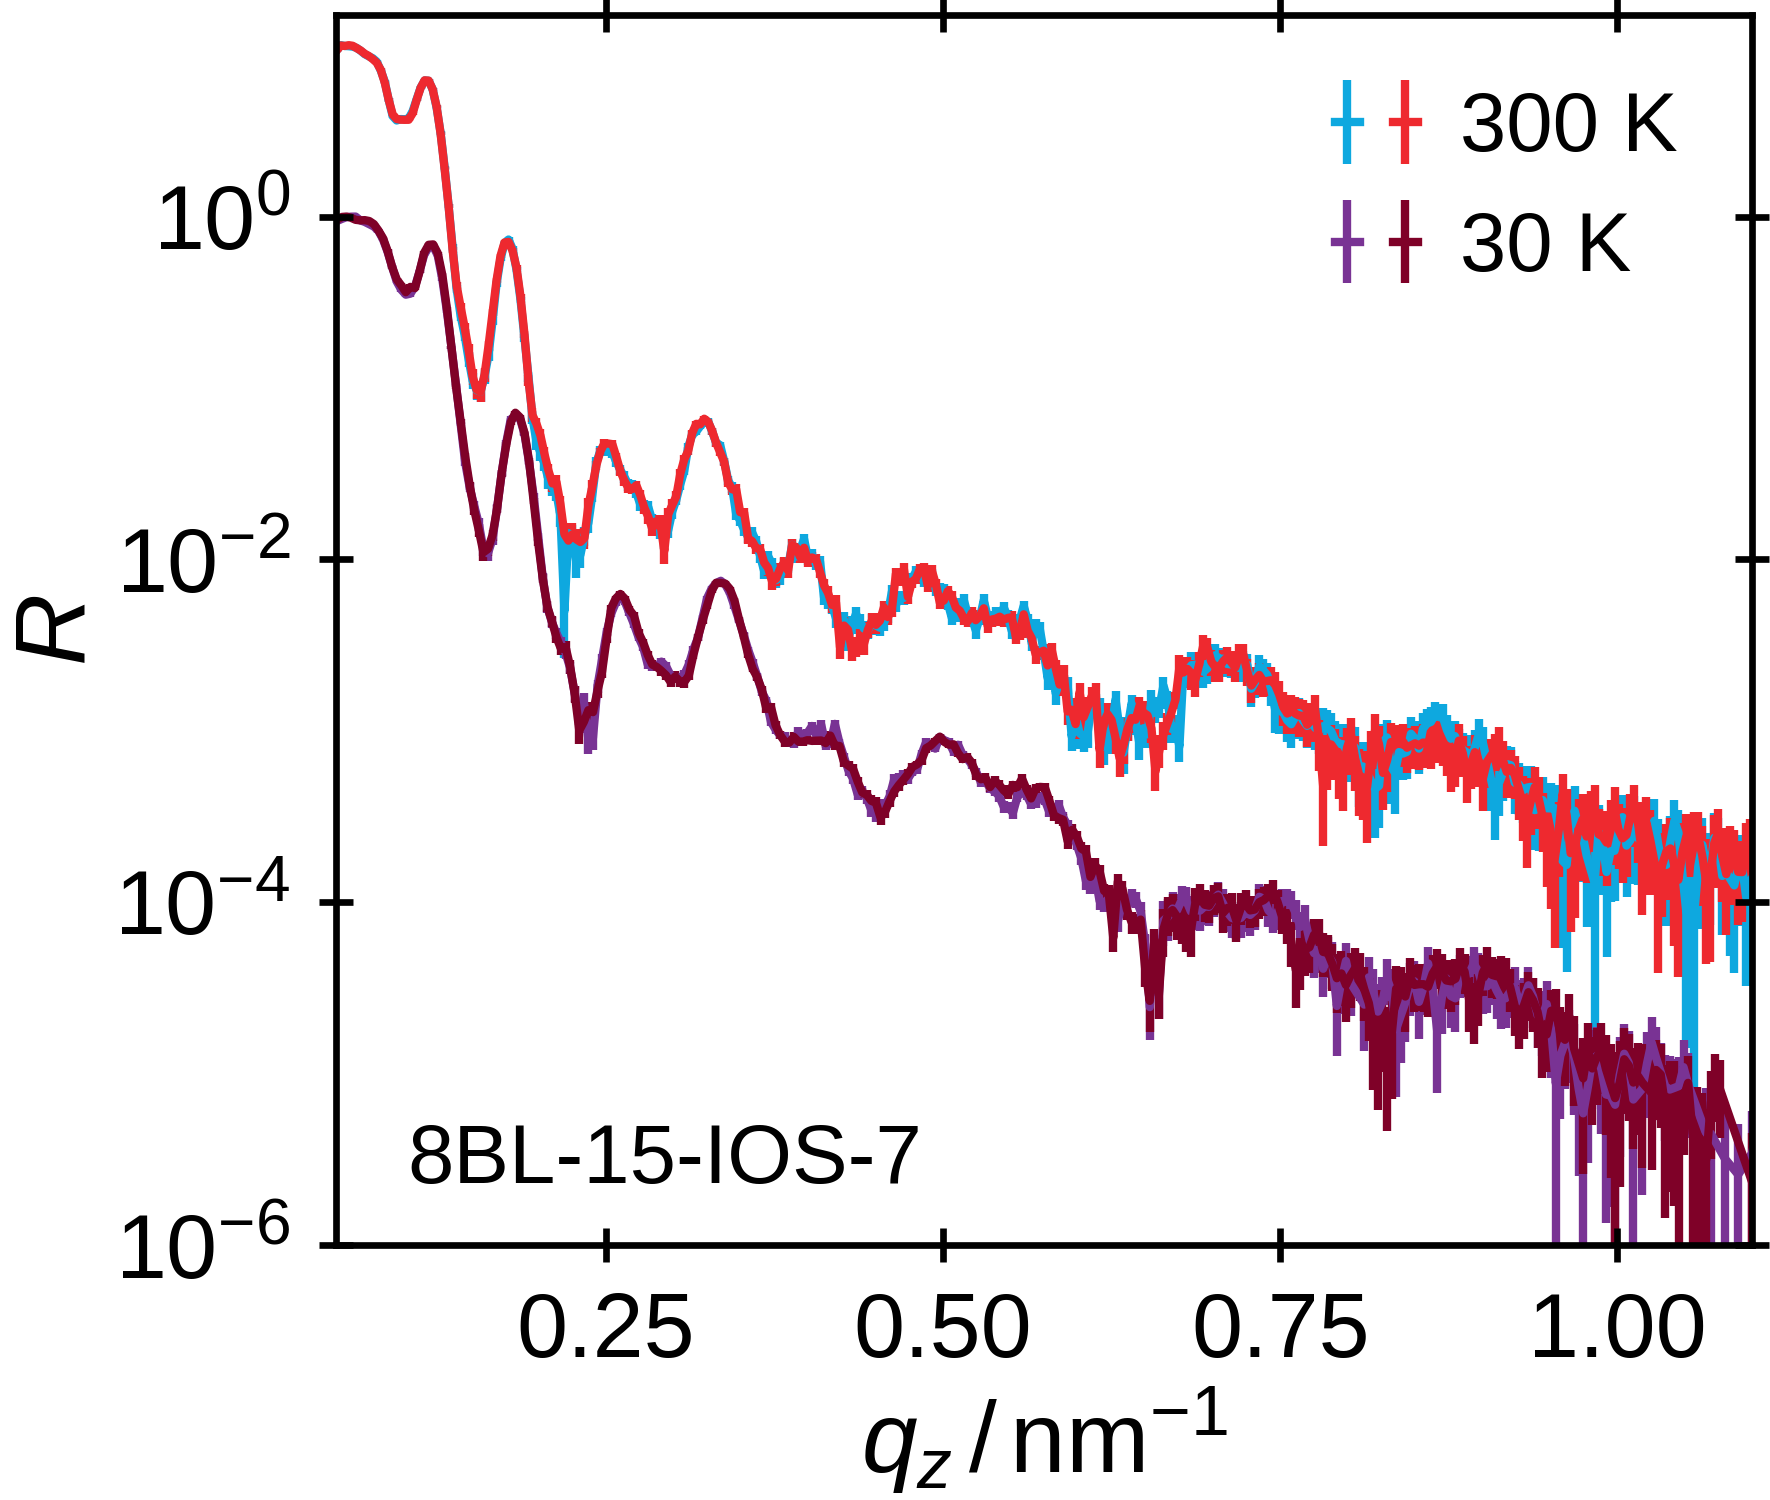
\includegraphics{looselyPackedNP_VerticalStructure_8BL-15-IOS-7_PNRCompare30K300K}
    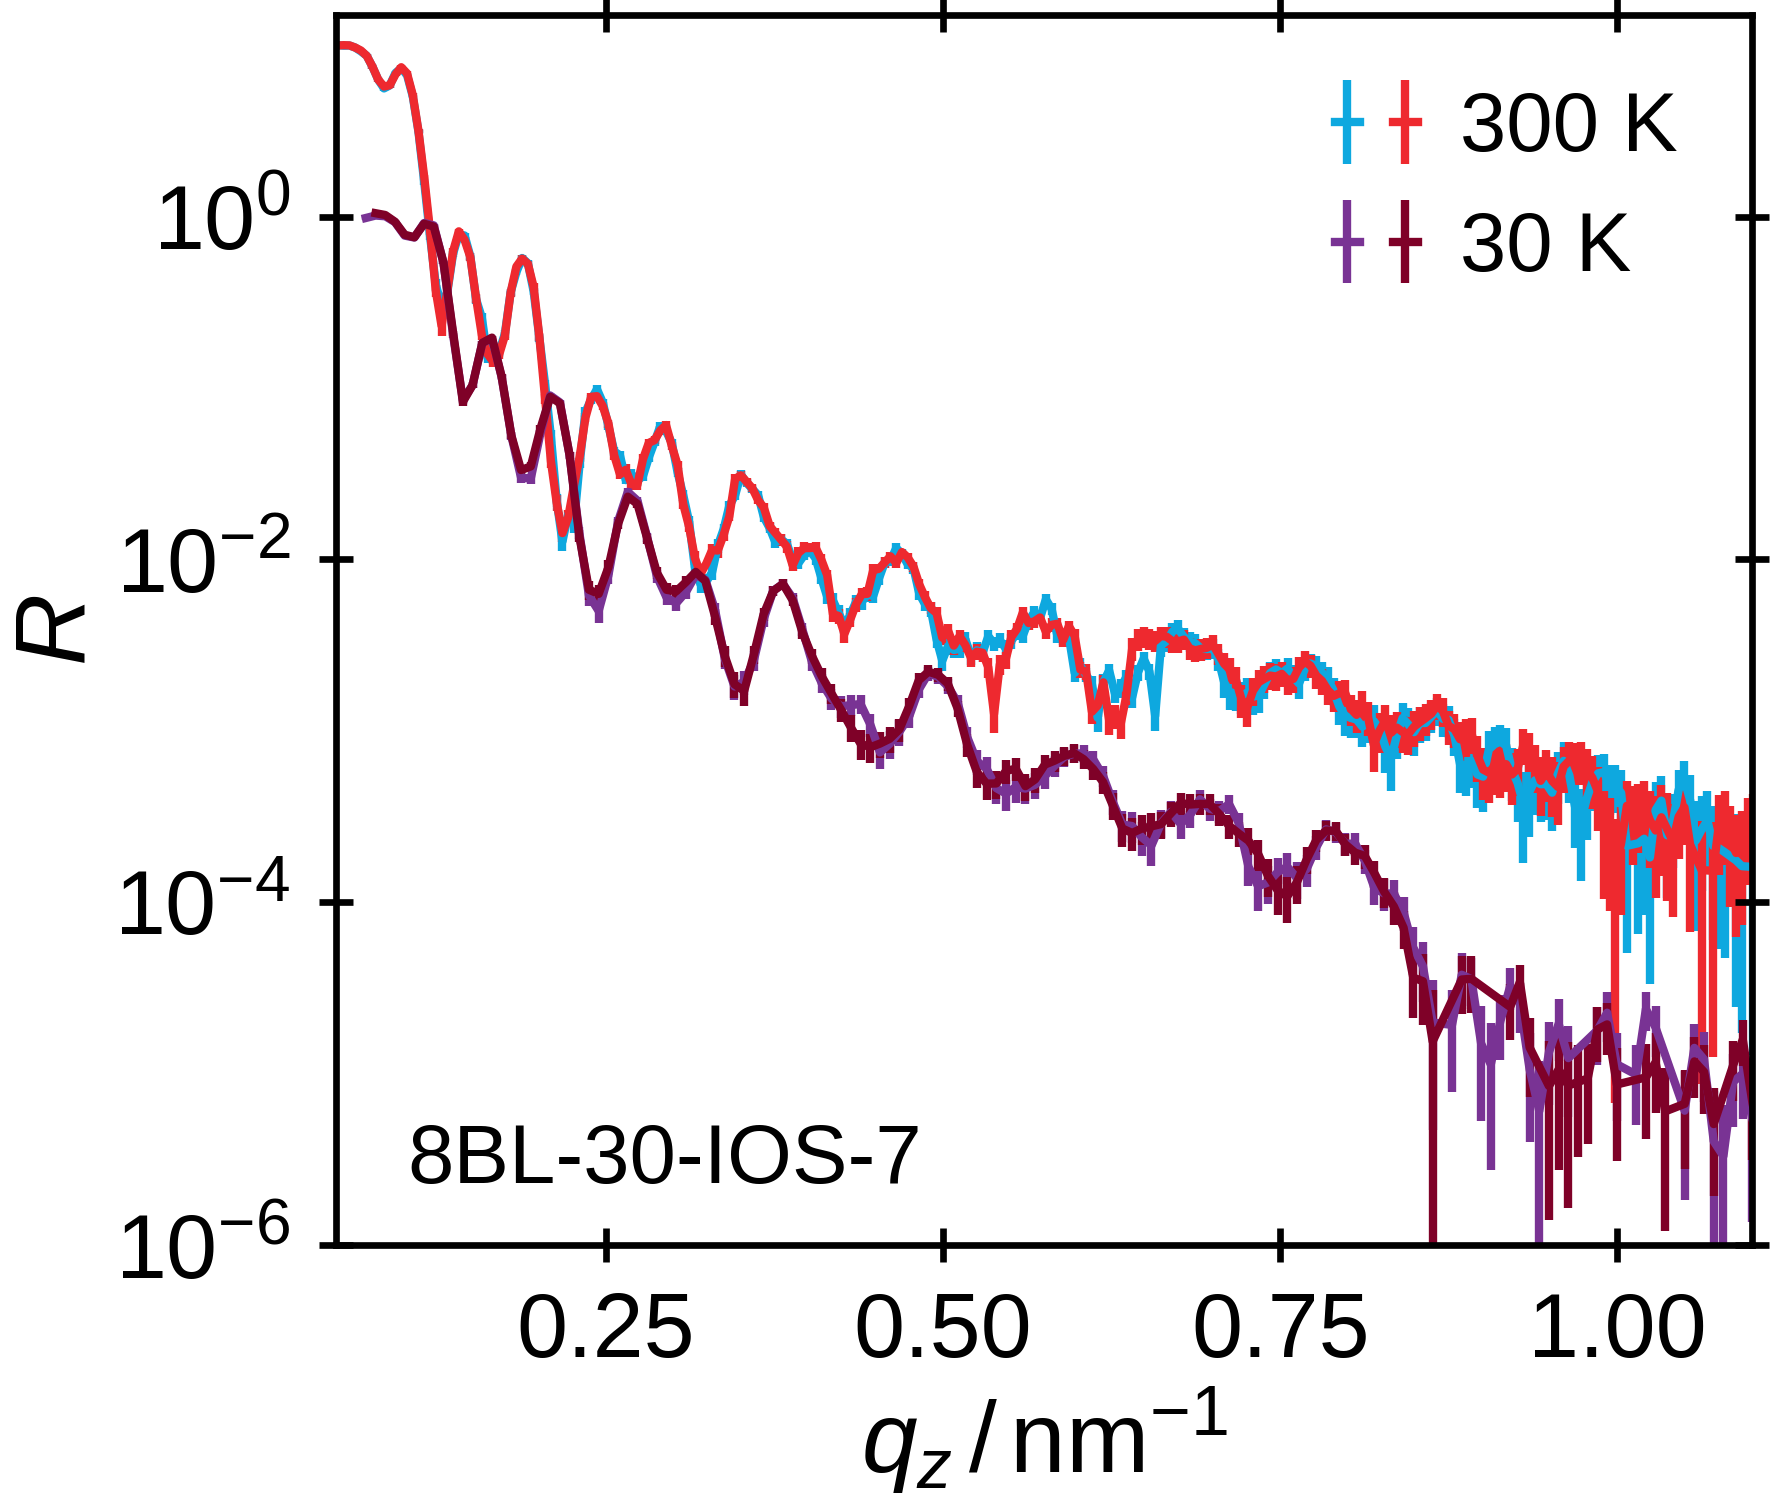
\includegraphics{looselyPackedNP_VerticalStructure_8BL-30-IOS-7_PNRCompare30K300K}
    \caption{\label{fig:looselyPackedNS:bilayerStacks:nr300K8BLIOS7}Neutron reflectivity data of the bilayer stacks 8BL-15-IOS-11 (left) and 8BL-40-IOS-11 (right) after footprint correction.}
  \end{figure}

  Furthermore, neutron reflectometry for all four samples was obtained at room temperature and $30 \unit{K}$ using the SuperADAM instrument at ILL and is shown in \reffig{fig:looselyPackedNS:bilayerStacks:nr300K8BLIOS11} for 8BL-x-IOS11 and in \reffig{fig:looselyPackedNS:bilayerStacks:nr300K8BLIOS7} for 8BL-x-IOS7 respectively.
  Looking at the room temperature measurements, similar to XRR, peaks are clearly visible in the reflectivity, which can be associated to the periodicity of the unit cell in the bilayer stacks.
  Remarkably, this is the case for the samples 8BL-x-IOS11, as well as for 8BL-x-IOS7, which showed no signal in X-ray reflectivity.
  It can be concluded that the structureless reflectivity of 8BL-x-IOS7 in XRR is mainly due to a contrast matching in the sample.
  For X-rays in the order of $1.54 \unit{\angstrom}$, the scattering length density of PMMA ($10.8 \cdot \unit{10^{-6} \angstrom^{-2}}$) and oleic acid ($8.52 \cdot \unit{10^{-6} \angstrom^{-2}}$) are in a similar order of magnitude, whereas for neutrons a large contrast is given between the two compounds with $1.059 \cdot \unit{10^{-6} \angstrom^{-2}}$ and $0.078 \cdot \unit{10^{-6} \angstrom^{-2}}$ respectively.
  If due loose packing, the average nanoparticle scattering length density is on a similar order of magnitude, no reflectivity can be studied, which is presumably the case for X-ray in the 8BL-x-IOS-7 samples.
  Using the sensitivity of neutrons to the nuclear structure instead of the electronic structure of the sample, better conditions are given for the study of the given sample class.

  The neutron reflectivities measured at $30 \unit{K}$ are shifted in comparison to the room temperature measurements towards higher $q$ values in all cases.
  The shift of the peaks in the reflectivity, with an increasing inter-peak distance translates in real space to reduction of the thickness for the bilayer unit cell.
  A shift of the critical edge to larger $q$ values furthermore translates to a higher average scattering length density of the sample, as the critical angle is directly proportional to the sample SLD.
  Both observations combine to the conclusion that the nanospheres have in all cases moved closed to one another in the loosely packed layers upon cooling, as was the case for the single spin-coated layer in \refsec{sec:looselyPackedNS:layers:xrr}.
  As for X-ray reflectivity, the peak positions have been evaluated to determine the thickness of a bilayer unit cell.
  The obtained lengths are tabulated in \reftab{tab:looselyPackedNP:bilayerStacks:reflPeriodLengths} together with the XRR result and the length scale from SEM for direct comparison.

  \begin{table}[tb]
    \centering
    \caption{\label{tab:looselyPackedNP:bilayerStacks:reflPeriodLengths}Average thickness of the bilayer stacks determined from the peaks in the reflectivities. Additionally, the period from SEM is shown for direct comparison.}
    \begin{tabular}{ c | l | l | l | l}
      \rule{0pt}{2ex} & $L^\mathrm{SEM} \, / \unit{nm}$ & $L^\mathrm{XRR} \, / \unit{nm}$ & $L^\mathrm{NR,\,300K}\, / \unit{nm}$ & $L^\mathrm{NR,\,30K}\, / \unit{nm}$ \\
      \hline
      \rule{0pt}{2ex} 8BL-15-IOS-11    & $63(5)$    & $91(3)$     & $78(1)$  & $76(1)$\\
      \rule{0pt}{2ex} 8BL-40-IOS-11    & $93(4)$    & $124(2)$    & $112(2)$ & $110(2)$\\
      \rule{0pt}{2ex} 8BL-15-IOS-7     & $50(4)$    &             & $86(1)$  & $83(1)$\\
      \rule{0pt}{2ex} 8BL-30-IOS-7     & $89(5)$    &             & $117(2)$ & $114(1)$\\
      \hline
    \end{tabular}
  \end{table}

  In all cases the cooling of the samples lead to a reduction of $2 - 3 \unit{nm}$ for each unit cell.
  For neutrons, the unit cells appear approximately $12 \unit{nm}$ smaller than when the sample is studied with X-rays.
  This can again be associated with the different contrast of the samples for X-rays and neutron scattering.
  As there is only a small contrast between the nanoparticle layers and the PMMA layers, depending on the packing density of the nanoparticles, the lines as to where the nanoparticle layer ends and the next PMMA layer starts are not well defined and therefore the unit cell appears enlarged for X-rays.

  The increased size of the period observed by neutrons in comparison to the length scale observed by SEM on the other hand can be argued with the measurement process in scanning electron microscopy.
  For one, the SEM micrograph is obtained after violently breaking the sample, which possibly distort the micrometer thick cross-section in the process.
  And for the other, an electron beam in scanning electron microscopy can burn and dissolve the organic PMMA compound partly and thereby lead to a collapse of the measured PMMA layer thickness.
  Therefore, the thickness by SEM is due to it's invasive nature more a rough estimate layer thickness and the results from the non-invasive neutron reflectivitiy are more trustworthy.

  A full quantitative evaluation of the X-ray and neutron reflectivity by the modeling of a scattering length density profile has not been achieved due to the high complexity of the sample and the large number of independent variables that are involved.
  Mastering this difficult task would allow otherwise to evaluate the thickness of the $16$ layers in the sample with depth resolution and is a necessary prerequisite to quantitatively evaluate the spin-density of the samples from polarized neutron reflectometry.

\end{document}